\documentclass[caret-main.tex]{subfiles}
\begin{document}
%-------------------------------------------%
\section{ROC Curves}

% What are ROC Cuves?

This type of graph is called a Receiver Operating Characteristic curve (or ROC curve.) It is a plot of the true positive rate against the false positive rate for the different possible cutpoints of a diagnostic test.

An ROC curve demonstrates several things:

It shows the tradeoff between sensitivity and specificity (any increase in sensitivity will be accompanied by a decrease in specificity).
The closer the curve follows the left-hand border and then the top border of the ROC space, the more accurate the test.
The closer the curve comes to the 45-degree diagonal of the ROC space, the less accurate the test.
The slope of the tangent line at a cutpoint gives the likelihood ratio (LR) for that value of the test. You can check this out on the graph above. Recall that the LR for T4 < 5 is 52. This corresponds to the far left, steep portion of the curve. The LR for T4 > 9 is 0.2. This corresponds to the far right, nearly horizontal portion of the curve.
The area under the curve is a measure of text accuracy.

\newpage
%--------------------------------------------%
\begin{figure}
\centering
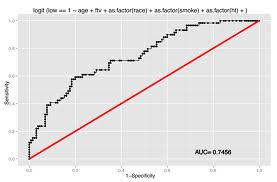
\includegraphics[width=0.7\linewidth]{./ROCcurve}
\caption{}
\label{fig:ROCcurve}
\end{figure}

%--------------------------------------------%
% http://stats.stackexchange.com/questions/24325/lorenz-curve-and-gini-coefficient-for-measuring-classifier-performance


\end{document}
